\chapter{Introduction}
\label{introduction}

\section{Overview}

The following environment is required:

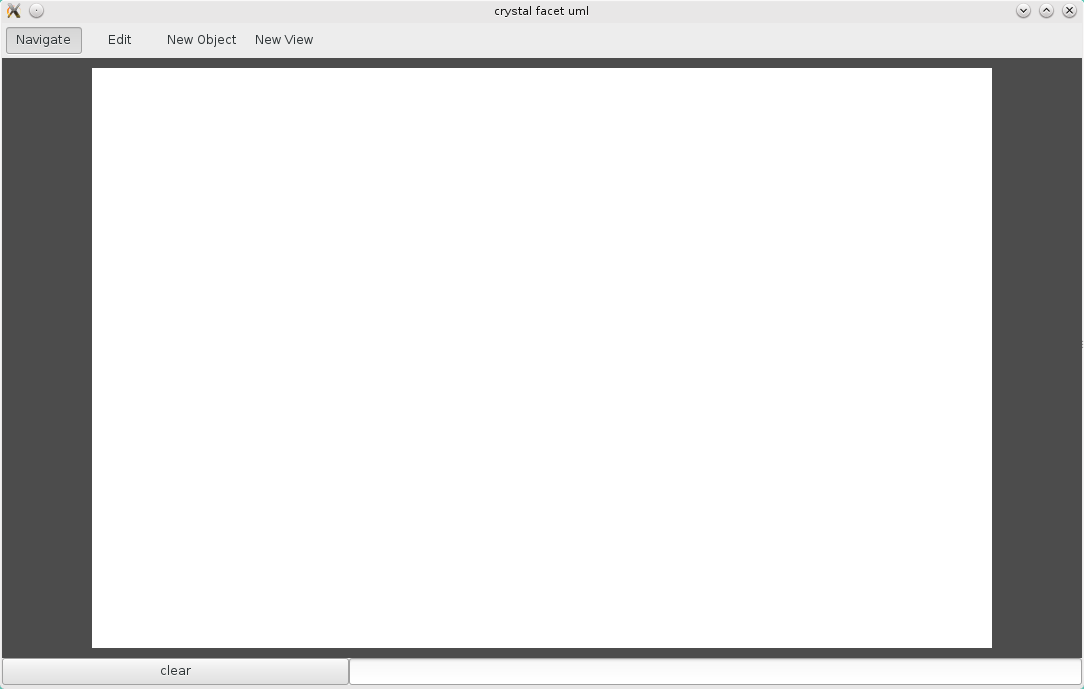
\includegraphics[width=10cm]{screenshot_1.png}




\includegraphics[width=2cm]{../../gui/source/resources/crystal_facet_uml}
%
\includegraphics[width=2cm]{../../gui/source/resources/crystal_facet_uml.pdf}
%\includegraphicshtml[width=2cm]{../../gui/source/resources/crystal_facet_uml.png}


crystal\_facet\_uml is a uml diagram drawing tool
that creates a set of consistent uml diagrams.

If started in graphical mode, it shows a window with
\begin{itemize}
\item toolbar on top,
\item drawing area in the center,
\item element configuration widgets below and
\item an optional notification bar at the bottom.
\end{itemize}

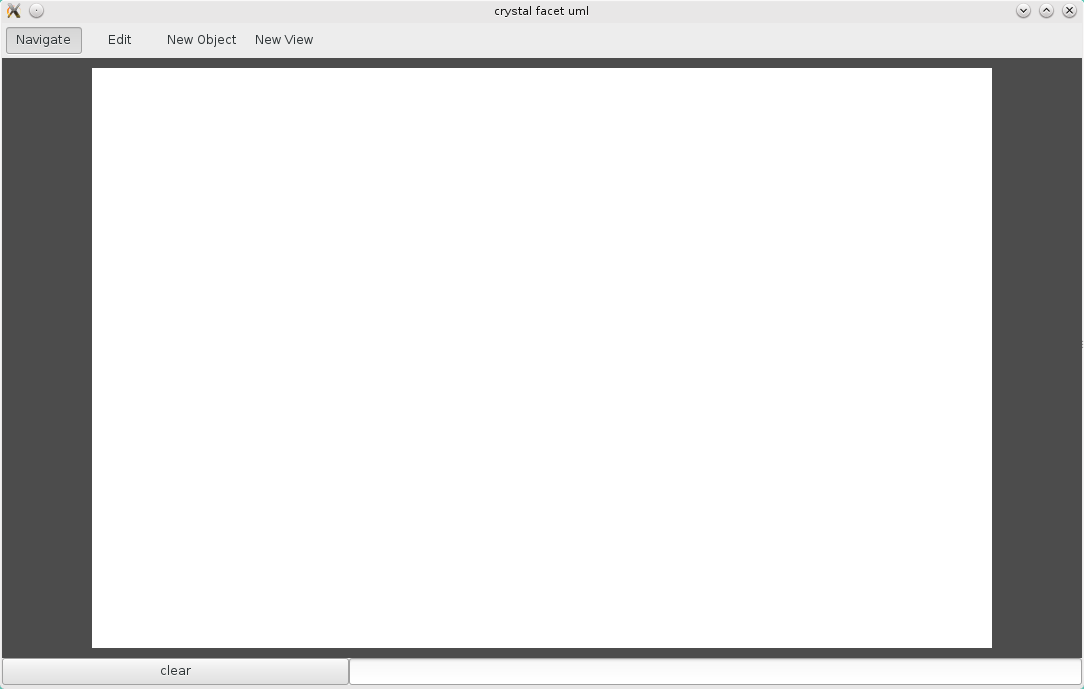
\includegraphics[width=10cm]{screenshot_1.png}

Additionally, crystal\_facet\_uml can be started from command line
to check and repair database files.
Run
code{.sh}
./crystal\_facet\_uml -h
endcode
to get a list of supported parameters.

